\documentclass{article}
\usepackage{enumerate, tikz, fancyhdr, framed, color}
\usepackage[margin=1.25in]{geometry}
\usepackage{amsmath}

% =============================================================

\pagestyle{fancy}
\definecolor{shadecolor}{gray}{0.95}
\lhead{Lucas Freitas and Emi Nietfeld}
\chead{} 
\rhead{\thepage} 
\lfoot{\small Computer Science 124} 
\cfoot{} 
\rfoot{\footnotesize Number Partition Problem} 
\renewcommand{\headrulewidth}{.3pt} 
\renewcommand{\footrulewidth}{.3pt}
\setlength\voffset{-0.25in}
\setlength\textheight{648pt}
\setlength\parindent{0pt}

% =============================================================

\begin{document}
\title{CS124 Programming Assignment 3\\\textsc{Number Partition Problem}}
\author{Lucas Freitas and Emi Nietfeld}

\maketitle

\thispagestyle{empty}

\section*{1. Dynamic Programming Approach to Partition Problem}

Here we present a pseudo-polynomial time algorithm for the number partition problem. Assume that the $n$ numbers to be partitioned sum up to some number $b$, our solution runs in time o($nb$).\\

We recognize the subproblem: for any number $k$, less than $b$, is there a partition of the first $j$ numbers that sum to $k$? We'll say P$(j, k)$ is true if there is a partition and false otherwise.\\

To answer this question we set up an $n$ by $b$ table of results, which stores the result of P$(j, k)$ for the row and column.\\

Let $i_1, i_2, i_3.... i_n$ be the series of input numbers.\\ 

For our base condition, we have:\\
\[
P(1, k)=
\begin{cases}
    true, &  i_1 = k.\\
    false, & \text{otherwise}.
\end{cases}
\]

We solve the following recurrence equation: \\
\[
P(j, k)=
\begin{cases}
    true, &  P(j-1, k) \text{ or } P(j-1, k - i_{j}).\\
    false, & \text{otherwise}.
  \end{cases}
\]
  
 Consider that any subset of the first $j$ numbers either includes $i_j$ or it does not. Therefore, there is only a subset that sums to $k$ if  and only if there is a subset \emph{without} $i_j$ that sums to $k$ \emph{or} that sums to $k - i_j$, so that $i_j$ is included. \\

To find the minimum residue, we fill in the above table diagonally and we locate the closest j to $b/2$ where $P(j)$ holds true.\\

To do this, we see that we are dividing $b$ into two groups, $x$ and $y$ where $x + y  = b$. The difference between the two groups (the residue, $r$.) Is the same as the difference between 2*$x$ and $b$. Therefore: 

\begin{center} 
$x - y = x - (b -x) = r$ 
$x = \frac{b + r}{2}$
\end{center}

Therefore, we see that having P($\frac{b + r}{2}$) be true implies there is a partition with residue $r$. We simply select the value for which $r$ is minimized and we have found the minimum residue, $(\frac{b}{2} - j)\cdot2$

We see that initialization, each step of the recursion, and checking for the minimum residue takes constant time. We perform one calculation for each entry in the table (for $1 \leq k \leq b$, $i \leq j \leq n$) for a total of O($nb$) calculations. 

\newpage
\section*{2. Karmarker-Karp in O($n\log{n}$) time} 
We sort the list, in descending order, in time O($n\log{n}$).\\ 

We then take the largest two elements off of the list and subtract them in time O(1).\\

We then insert the result back into the list, which using binary search takes O($\log{n}$) time. \\ 

We do this until there's only one element in the list, the residual. This is O($n$) repetitions, for a total running time of O($n\log{n}$)\\
    
\section*{3. Implementation} 
We wrote our programming assignment using Python. While we may not have been as fast (particularly for generating the random solutions) as C, we found its performance perfectly acceptable. Our choice of language illustrated very nicely the tradeoffs between program speed and programmer time. The latter was infinitely more valuable in this case.\\

For all of the algorithms, we found it useful to modify lists in place. We cut down on our run time on some lists by stopping when the residual is zero. We also optimized hill climbing based on the realization that we didn't need to continually residual over the entire list, only update our running count based on the elements we changed.\\

To improve the running time of Karmarkar-Karp, we used a maximum heap in order to quickly take the largest elements and improve the running time. Through sorting the list of incoming integers as we generated the random pre-partitions we were able to do this step in a single pass. 
\newpage
\section*{4. Results} 
\subsection*{4.1. Performance graphs}

Put in the time results. \\ 

Running the program for $50$ tests with $2500$ iterations for each iterative algorithm, we get the following minimum residue graph for each of the algorithms:
\begin{center}
    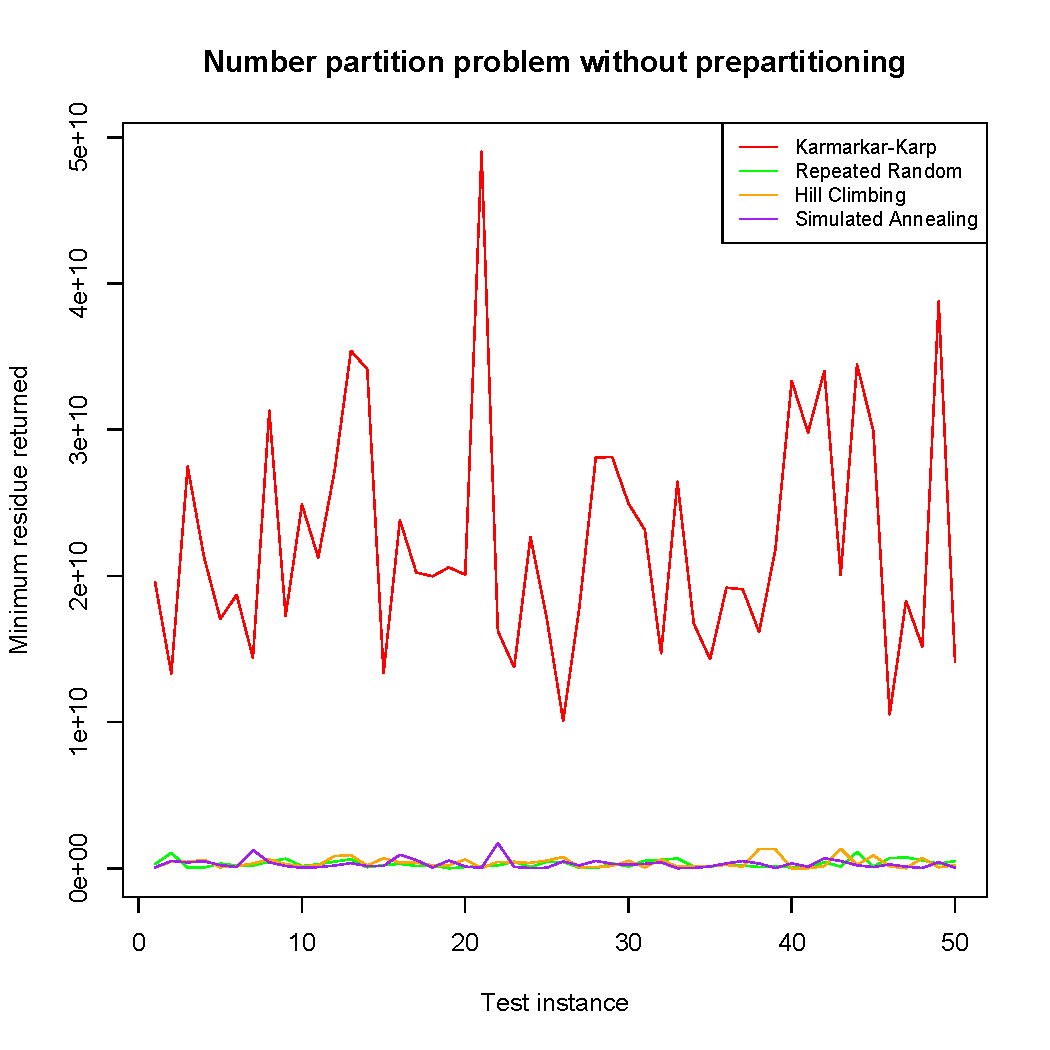
\includegraphics[width=0.45\textwidth]{graph1} 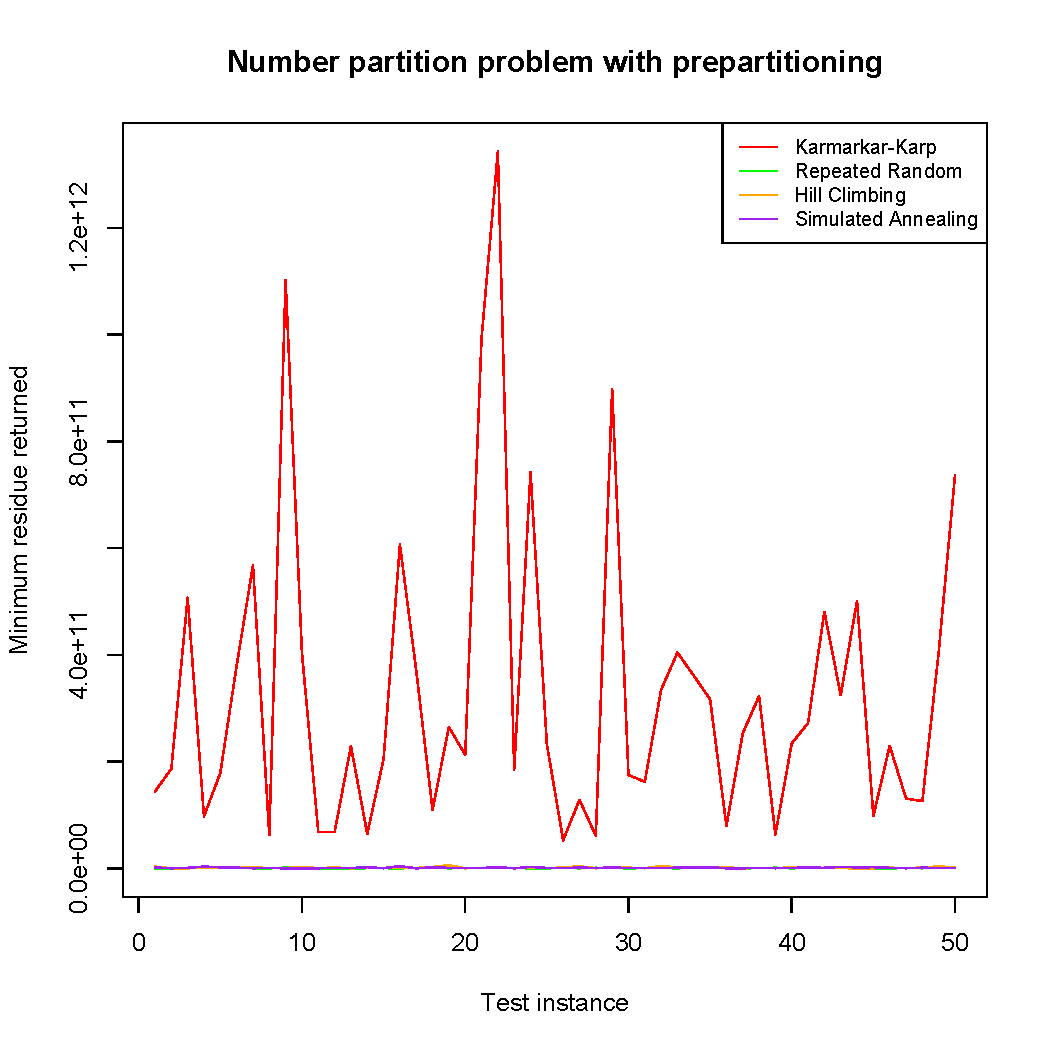
\includegraphics[width=0.45\textwidth]{graph1_pre}\\
\end{center}
It is easy to see that Karmarkar-Karp has much lower performance than all the other algorithms, so zooming just on the other three:
\begin{center}
    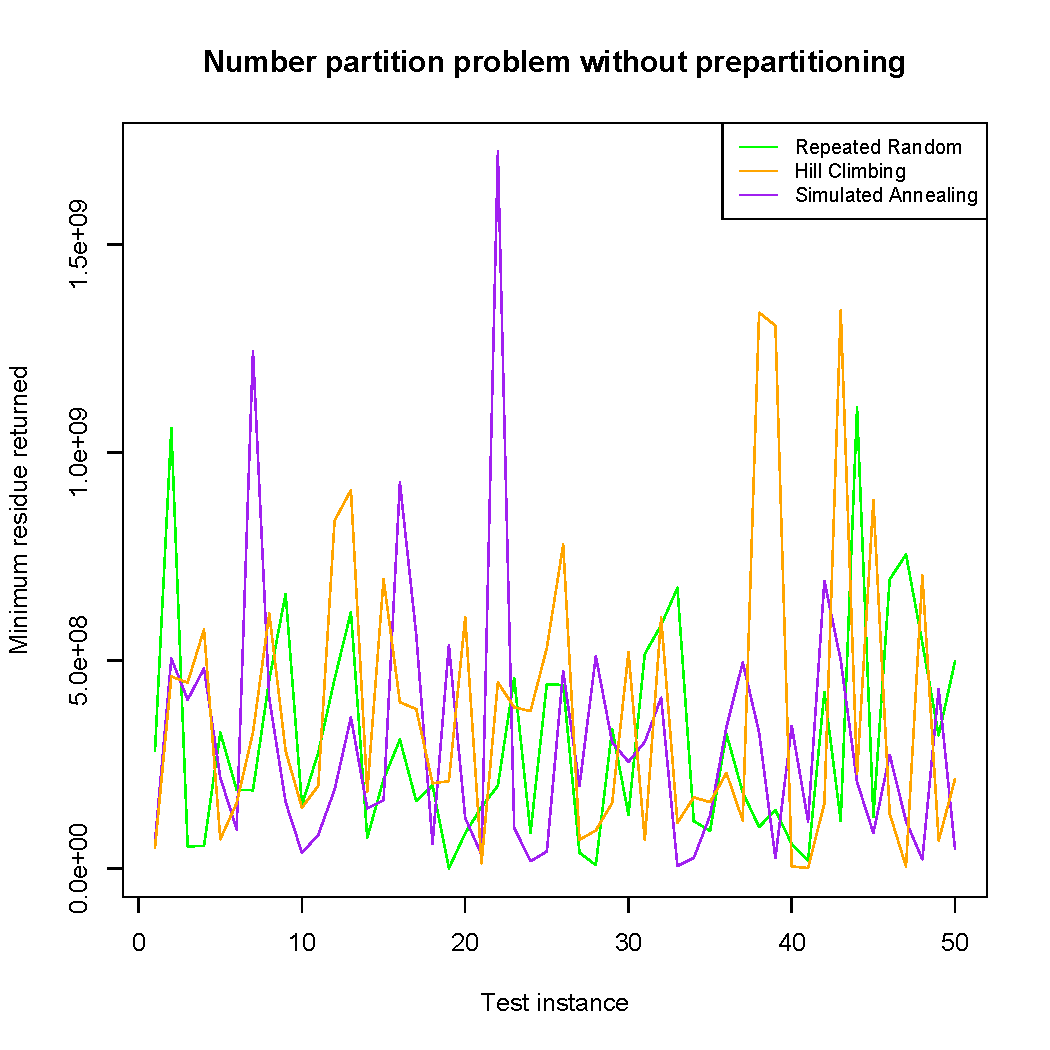
\includegraphics[width=0.45\textwidth]{graph2} 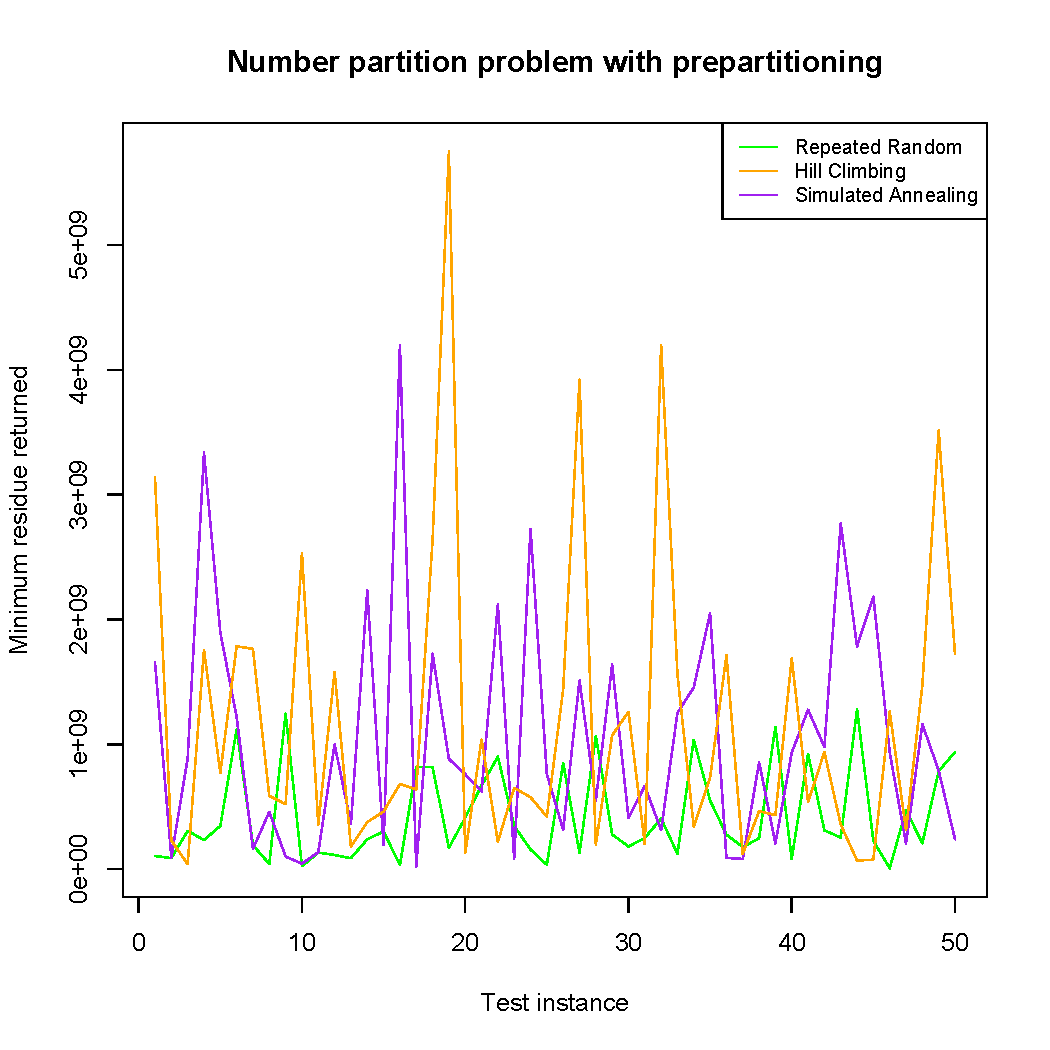
\includegraphics[width=0.45\textwidth]{graph2_pre}
\end{center}

\subsection*{4.2. Performance ranking}
    With prepartitioning, we noticed that Repeated Random yields lower avereage residues ($421736561$), followed by Simulated Annealing ($1046074505$), Hill Climbing ($1168005816$), and Karmarkar-Karp ($329528709576$).\\
    
    Without prepartitioning, the ranking changes to Simulated Annealing with the lowest avereage residue ($306161582$), followed by Repeated Random ($309641932$), Hill Climbing ($379177990$), and Karmarkar-Karp ($22388809139$)

\newpage
\section*{5. Discussion}
\subsection*{5.1. Karmarkar-Karp}
The results, both with or without pre-partioning, are very dramatic. As we see, Karmarkar produces both a much more volatile and much greater ammound of residual compared to the other algorithms.\\ 

We hypothesize that this is because the algorithm does poorly with larger numbers relative to the size of the list. Prepartitioning both makes some numbers larger \emph{and} makes the list shorter, magnifying this effect. \\

The relative volatility of Karmarkar can also be seen as resulting from Karmarkar's sensitivity to the various sizes of numbers. When numbers have a greater variance, Karmarkar results in a worse residue.\\
p
Karmarkar's performance when using prepartitioning was specially oor , leading to an average minimum residual $20$ times larger than for without prepartitioning ($4\cdot10^{11}$ as opposed to $2\cdot10^{10}$).\\

Considering that Karmarkar's algorithm runs in approximately $0.0009$ seconds for each test with prepartitioning, and $0.0012$ seconds without prepartitioning, and both times are fairly low and close to each other, it seems that if we decide to in fact use Karmarkar-Karp for the problem, we shouldn't simplify the problem even more by using prepartitioning.\\

Instead, we should let the algorithm run $0.0003$ longer for each test and get an answer $20$ closer to the optimum.
.
\subsection*{5.2. Hill Climbing, Repeated Random and Simulated Annealing}
When plotted against Karmarkar, these three algorithms seem to have nearly identical average performance. In fact, they all yield an average residual of approximately $5\cdot10^8$ without prepartitioning and $10^9$ when prepartitioning. While this is double the residual, it's in the same order of magnitude. \\

We also see some improvement on the time of execution of repeated random when using prepartitioning ($3.70$ versus $5.42$), although there is no significant change in time performance for Hill Climbing or Simulated Annealing. That is intuitive, though. Repeated random draws a new solution every time, so when we reduce the size of the list of numbers by doing prepartitioning, repeated random has to generate way less random numbers, and it executes much faster.\\
 
As we see, repeated random was both the least volatile and the most optimal of all of our algorithms. It also was the least negatively impacted by pre-partitioning. Intuitively, this makes sense: the randomness of pre-partitioning is essentially equivalent to the randomness of repeated random solution, so just one added layer of randomness, in which we hope to still get a good solution, doesn't impact the performance of repeated random as much as the other algorithms, although the performances are still quite close.\\

Repeated random also took, by far, the longest. While each step of hill climbing and simulated annealing could be performed in constant time, each round of repeated random took time O($n$).\

Simulated Annealing was very slightly faster than repeated random without pre-partitioning and was close behind without pre-partitioning. To a lesser extent than for repeated random, the randomness of pre-partitioning is similar to the "hot" stage of the annealing algorithm.\\

It would be very interesting to compare simulated annealing cooling factors over the number of iterations. We imagine that simulated annealing works especially well with our current cooling scheme since we have so many repetitions.\\

Not surprisingly, simulated annealing outperformed Hill Climbing. When we tested Hill Climbing, we noted that the residue changed very few times, suggested that it "got stuck" very early on and stayed stuck, to the point where we thought there was an error in our code. Looking at the results over all fifty tests, we note that hill climbing has quite a bit of variation. It seems to suggest that we either "lock" in a pretty good solution or miss it.\\

We estimate that hill climbing might outperform these other algorithms if we were only allowed to perform a much smaller number of repetitions.\\

\emph{An aside on pre-partitioning}

We also noted during testing that pre-partitioning on small list made it significantly slower while on longer list it sped up the run time. This makes sense as a result of constant factors. \\

\section*{6. Karmarkar Karp as a Starting Point}
One easy extension of Karmarkar-Karp is to run the algorithm for a certain number of rounds and use the result as an initial partitioning for any of the other algorithms.\\

We would expect that this would yield more accurate residuals, in general, then random pre-partitioning, but would also take longer. Also, in the case of numbers that are very large compared to the size of the list, it would also do poorly, as we've seen Karmarkar-Karp, in general to do. \\

As in the Complete Karmarkar-Karp algorithm, we could also try running Karmarkar-Karp while keeping track of the partitions (by keeping track of their sum.) With this information, we could create a binary tree and then, given enough time, find the optimal solution. 
\end{document}
 
